% !LW recipe=pdflatex dos veces
% Manual de usuario de la aplicación de chat.
% Compilar con: latexmk -pdf manual_usuario.tex
\documentclass[12pt, a4paper]{article}

\usepackage[spanish]{babel}
\usepackage[utf8]{inputenc}
\usepackage[T1]{fontenc}
\usepackage[margin=2.5cm]{geometry}
\usepackage{helvet}
\renewcommand{\familydefault}{\sfdefault}
\usepackage{setspace}
\usepackage{graphicx}
\usepackage{float}
\usepackage{xcolor}
\usepackage{fancyhdr}
\usepackage{wallpaper}
\usepackage[absolute,overlay]{textpos}
\usepackage{enumitem}
\usepackage{hyperref}
\usepackage{xurl}
\usepackage[varqu]{zi4}
\usepackage{listings}
\usepackage[most]{tcolorbox}

% Código: los bloques van en un cuadro de terminal con los colores del tema
% oscuro de Visual Studio Code, y el código dentro del texto, en otro color.
\definecolor{ideFondo}{HTML}{1E1E1E}
\definecolor{ideBarra}{HTML}{2D2D30}
\definecolor{ideBorde}{HTML}{3C3C3C}
\definecolor{ideTexto}{HTML}{D4D4D4}
\definecolor{ideTitulo}{HTML}{BBBBBB}
\definecolor{ideOrden}{HTML}{DCDCAA}
\definecolor{ideSubOrden}{HTML}{569CD6}
\definecolor{ideOpcion}{HTML}{9CDCFE}
\definecolor{ideCadena}{HTML}{CE9178}
\definecolor{ideVariable}{HTML}{4FC1FF}
\definecolor{codigoEnLinea}{HTML}{C7254E}

\lstdefinelanguage{consola}{
  sensitive=true,
  alsoletter={-.:},
  morekeywords=[1]{py,pip,ollama,scrapy},
  morekeywords=[2]{venv,install,pull,runspider},
  morekeywords=[3]{-m,-e,-O},
  morekeywords=[4]{$env:TFG_DESCARGAR_MODELO},
  morestring=[b]",
  morestring=[b]',
}

\newtcblisting{consola}{
  enhanced, listing only,
  colback=ideFondo, colframe=ideBorde, boxrule=0.6pt, arc=3pt,
  left=10pt, right=10pt, top=6pt, bottom=6pt,
  title={\ttfamily\footnotesize TERMINAL\quad PowerShell},
  colbacktitle=ideBarra, coltitle=ideTitulo, toptitle=2pt, bottomtitle=2pt,
  listing options={
    language=consola,
    basicstyle=\footnotesize\ttfamily\color{ideTexto},
    keywordstyle={[1]\color{ideOrden}},
    keywordstyle={[2]\color{ideSubOrden}},
    keywordstyle={[3]\color{ideOpcion}},
    keywordstyle={[4]\color{ideVariable}},
    stringstyle=\color{ideCadena},
    columns=fullflexible, keepspaces=true, showstringspaces=false,
    breaklines=true, upquote=true, aboveskip=0pt, belowskip=0pt,
  },
}

\let\textttOriginal\texttt
\renewcommand{\texttt}[1]{\textttOriginal{\textcolor{codigoEnLinea}{#1}}}

\hypersetup{
  colorlinks=true,
  linkcolor=blue,
  urlcolor=cyan,
  pdftitle={Manual de usuario de la aplicación de chat},
  pdfauthor={Samuel Blanco Palmero},
}

\definecolor{naranja}{RGB}{198,97,21}

\setlength{\parskip}{1em}
% Inconsolata es más ancha que la letra por defecto: sin holgura, una línea
% con un nombre de fichero no encuentra dónde cortar y se sale del margen.
\setlength{\emergencystretch}{2em}
\pagestyle{fancy}
\fancyhf{}
\fancyhead[L]{{\color{gray}Samuel Blanco Palmero}}
\fancyhead[R]{{\color{gray}Manual de usuario}}
\fancyfoot[L]{{\color{gray}Escuela Politécnica Superior de Jaén}}
\fancyfoot[R]{{\color{gray}\thepage}}
\renewcommand{\footrulewidth}{1pt}
\renewcommand{\spanishcontentsname}{Tabla de contenidos}

\begin{document}

% ---------- Portada: la misma plantilla que la memoria ----------
\thispagestyle{empty}
\ULCornerWallPaper{1}{../memoria/imagenes/portada.pdf}
\begin{textblock*}{18.45cm}(1.4cm,12cm)
  \centering
  {\fontsize{30}{40}\selectfont \textbf{\color{naranja}Manual de usuario de la aplicación de chat}}
  \vspace{.4cm}

  {\fontsize{12}{16}\selectfont Trabajo Fin de Grado: Sistema de información y recomendación de titulaciones oficiales de la UJA para estudiantes de secundaria}
  \vspace{.2cm}

  {\fontsize{16}{21}\selectfont Autor: Samuel Blanco Palmero}

  {\fontsize{16}{21}\selectfont Grado en Ingeniería Informática}

  {\fontsize{12}{10}\selectfont Director: Juan Carlos Cuevas Martínez}
  \vspace{-.4cm}

  {\fontsize{12}{10}\selectfont Departamento del director: Informática}

  \vspace{0.3cm}
  {\fontsize{16}{21}\selectfont Fecha: 28/10/2026}
\end{textblock*}
~
\clearpage
\ClearWallPaper

\onehalfspacing
\tableofcontents
\clearpage

% ---------------------------------------------------------------
\section[Qué es el asistente]{Qué es el asistente}



El Asistente Virtual de Titulaciones es una aplicación de chat pensada para ayudarte si estás en Bachillerato, en Formación Profesional o simplemente estás interesado en entrar en alguna titulación universitaria. Responde a tus preguntas sobre los grados que se imparten en la Escuela Politécnica Superior de Jaén (EPSJ) de la Universidad de Jaén. Funciona con una técnica llamada RAG (generación aumentada por recuperación), en la que primero busca en la información de la Escuela y después un modelo de lenguaje escribe la respuesta a partir de lo que ha encontrado.

Las respuestas salen de la información oficial que publica la propia Escuela en su web, como los planes de estudios, las guías docentes de las asignaturas, las menciones y las salidas profesionales. Con esa información el asistente puede contarte qué asignaturas hay en cada curso, cuántos créditos ECTS tiene cada una, qué se ve en ellas, de qué podrás trabajar al terminar o qué titulaciones encajan con lo que te gusta.

Este asistente es un Trabajo Fin de Grado y no un servicio oficial de la Universidad de Jaén. Sus respuestas las escribe en el momento un modelo de lenguaje, y por eso alguna vez pueden tener errores. Antes de tomar una decisión importante, comprueba siempre la información en la web oficial de la Escuela.

% ---------------------------------------------------------------
\section{Puesta en marcha}\label{sec:puesta}

En este apartado se explica qué necesitas y qué pasos hay que seguir para instalar el asistente y ponerlo en marcha en tu ordenador. Si ya lo tienes funcionando, puedes pasar directamente a la Sección~\ref{sec:pantalla}, que explica cómo usarlo.

\subsection{Requisitos del sistema}

Para que todo funcione necesitas tener instalado lo siguiente:

\begin{itemize}
  \item \textbf{Python 3.13}.
  \item \textbf{Ollama}, el programa que ejecuta el modelo de lenguaje en tu propio ordenador, con el modelo \texttt{gemma3:12b} ya descargado (ocupa unos 8,1~GB en disco). Cuando está cargado ocupa unos 8,9~GB de memoria: Ollama pone en la tarjeta gráfica lo que cabe y el resto va a la RAM. En el equipo de pruebas fueron 3,3~GB en la tarjeta y 5,6~GB en la RAM.
  \item El modelo de incrustaciones \texttt{intfloat/multilingual-e5-small}, que es el que permite buscar los textos por su significado. Ocupa unos 0,5~GB en disco y otros 0,5~GB de RAM cuando está cargado. Se descarga la primera vez que se construye el índice.
\end{itemize}

Los tiempos de respuesta se han medido en un portátil con 16~GB de memoria RAM y una tarjeta gráfica NVIDIA GeForce RTX 3060 con 6~GB de memoria. Es el equipo con el que se ha probado el asistente, no unos requisitos mínimos.

\subsection[Instalación y preparación de los datos]{Instalación y preparación de los datos}\label{sec:instalacion}

Tienes las instrucciones completas en el fichero \texttt{README.md} del repositorio\footnote{\url{https://github.com/samubp10/tfg-recomendador-uja}} y en \texttt{docs/\allowbreak instalacion.md}. En Windows, los comandos que hay que ejecutar desde la carpeta del proyecto son:

\begin{consola}
py -m venv .venv
.venv\Scripts\activate
pip install -e ".[dev,index]"
ollama pull gemma3:12b
\end{consola}

Los datos no vienen incluidos en el repositorio; se generan con la ejecución del sistema. Antes de construir el índice por primera vez tienes que permitir la descarga del modelo de incrustaciones con la variable de entorno \texttt{TFG\_DESCARGAR\_MODELO=1}, que es la tercera línea del bloque de abajo. El primer comando descarga la información directamente de la web de la EPSJ, así que solo hace falta ejecutarlo la primera vez y cuando quieras actualizar los datos:

\begin{consola}
scrapy runspider src/tfg_uja/extraccion/grados_spider.py -O data/grados.json
py -m tfg_uja.indexacion.chunker data/grados.json data/chunks.json
$env:TFG_DESCARGAR_MODELO = '1'
py -m tfg_uja.indexacion.indexer data/chunks.json data/indice_lance
\end{consola}

\subsection[Arrancar el asistente]{Arrancar el asistente}\label{sec:arrancar}

Con Ollama en marcha (en Windows suele arrancar solo y quedarse en segundo plano), el asistente se arranca con:

\begin{consola}
py -m tfg_uja.aplicacion.servidor
\end{consola}

Cuando en la terminal aparezca el mensaje \texttt{Asistente en http://127.0.0.1:8000}, abre esa dirección en tu navegador. Para parar el proceso, pulsa \texttt{Ctrl+C} en la terminal.

El asistente solo funciona en tu propio ordenador y atiende las preguntas de una en una. Es un prototipo para usarlo en local.

% ---------------------------------------------------------------
\section[La pantalla principal]{La pantalla principal}\label{sec:pantalla}

Al abrir el asistente en el navegador verás la pantalla de la Figura~\ref{fig:inicio}. De arriba abajo, tiene estas partes:

\begin{enumerate}
  \item \textbf{Cabecera:} La parte verde de arriba contiene el escudo de la Universidad de Jaén, el nombre del asistente y, debajo, el trabajo y el autor.
  \item \textbf{Conversación:} Es el cuerpo de la aplicación, la parte central. Empieza con un saludo y en ella van apareciendo tus preguntas y las respuestas.
  \item \textbf{Preguntas sugeridas:} Encima del cuadro de texto hay unos botones con ejemplos de preguntas. Si pulsas uno, la pregunta se envía directamente. Después de cada respuesta cambian: la mitad de ellas siguen con la titulación por la que estás preguntando y la otra mitad te propone conocer otras de la Escuela.
  \item \textbf{Cuadro de texto:} Es donde escribes tu pregunta, con el botón de enviar a la derecha.
  \item \textbf{Avisos:} Son consejos que te recuerdan qué puedes preguntar, que el modelo de lenguaje se puede equivocar, y llevan el enlace a la política de privacidad.
\end{enumerate}

\begin{figure}[H]
  \centering
  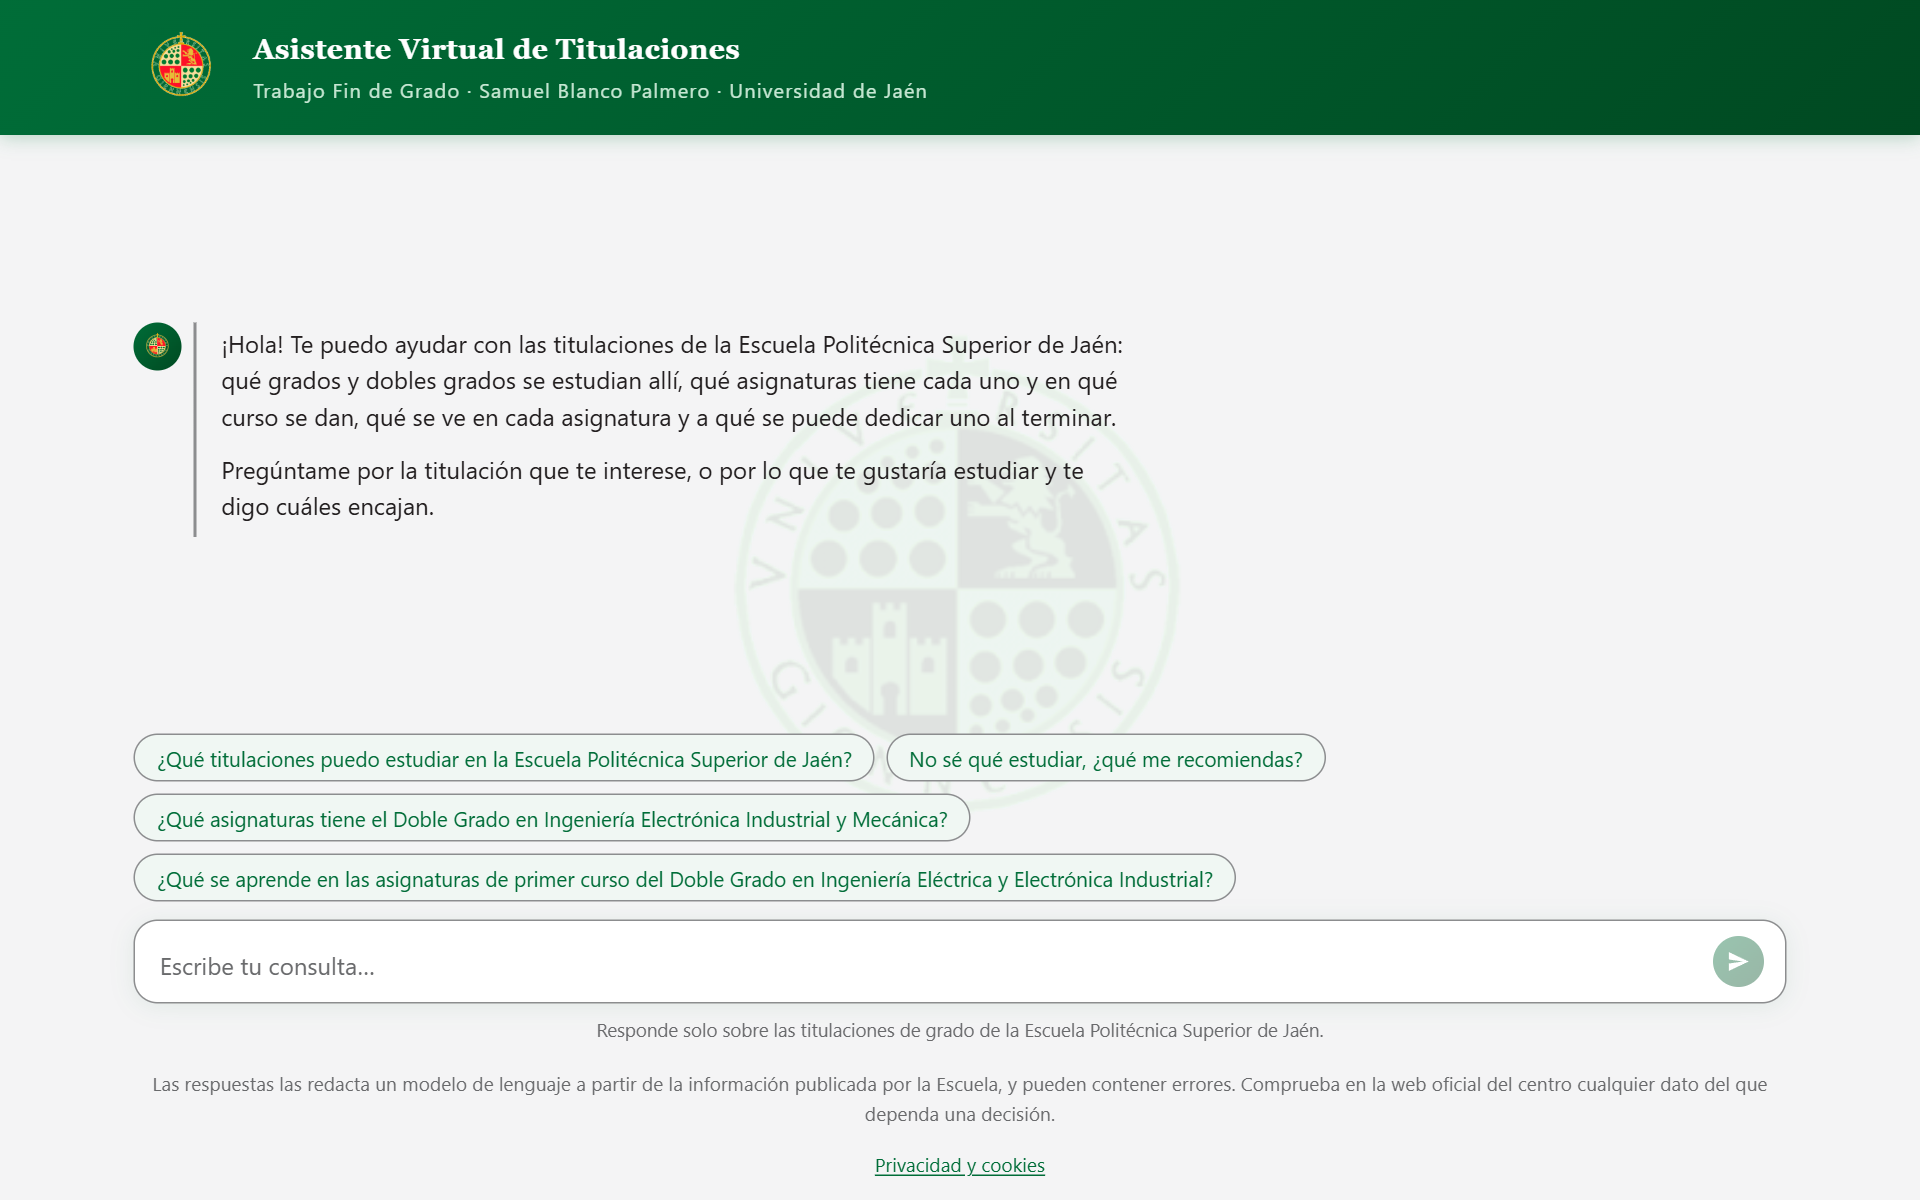
\includegraphics[width=\textwidth]{capturas/01_inicio.png}
  \caption{Pantalla principal de la aplicación.}
  \label{fig:inicio}
\end{figure}

% ---------------------------------------------------------------
\section[Cómo hacer una pregunta]{Cómo hacer una pregunta}

Para hacer una pregunta, escríbela en el cuadro de abajo y pulsa Intro o el botón de enviar (Figura~\ref{fig:escrita}). Si quieres escribirla en varias líneas, usa Mayús+Intro para saltar de línea.

Para que el asistente encuentre mejor lo que buscas, di de qué titulación o asignatura hablas. Por ejemplo, «¿Qué salidas profesionales tiene el Grado en Ingeniería Informática?» funciona mucho mejor que algo tan general como «¿de qué podré trabajar?».

\begin{figure}[H]
  \centering
  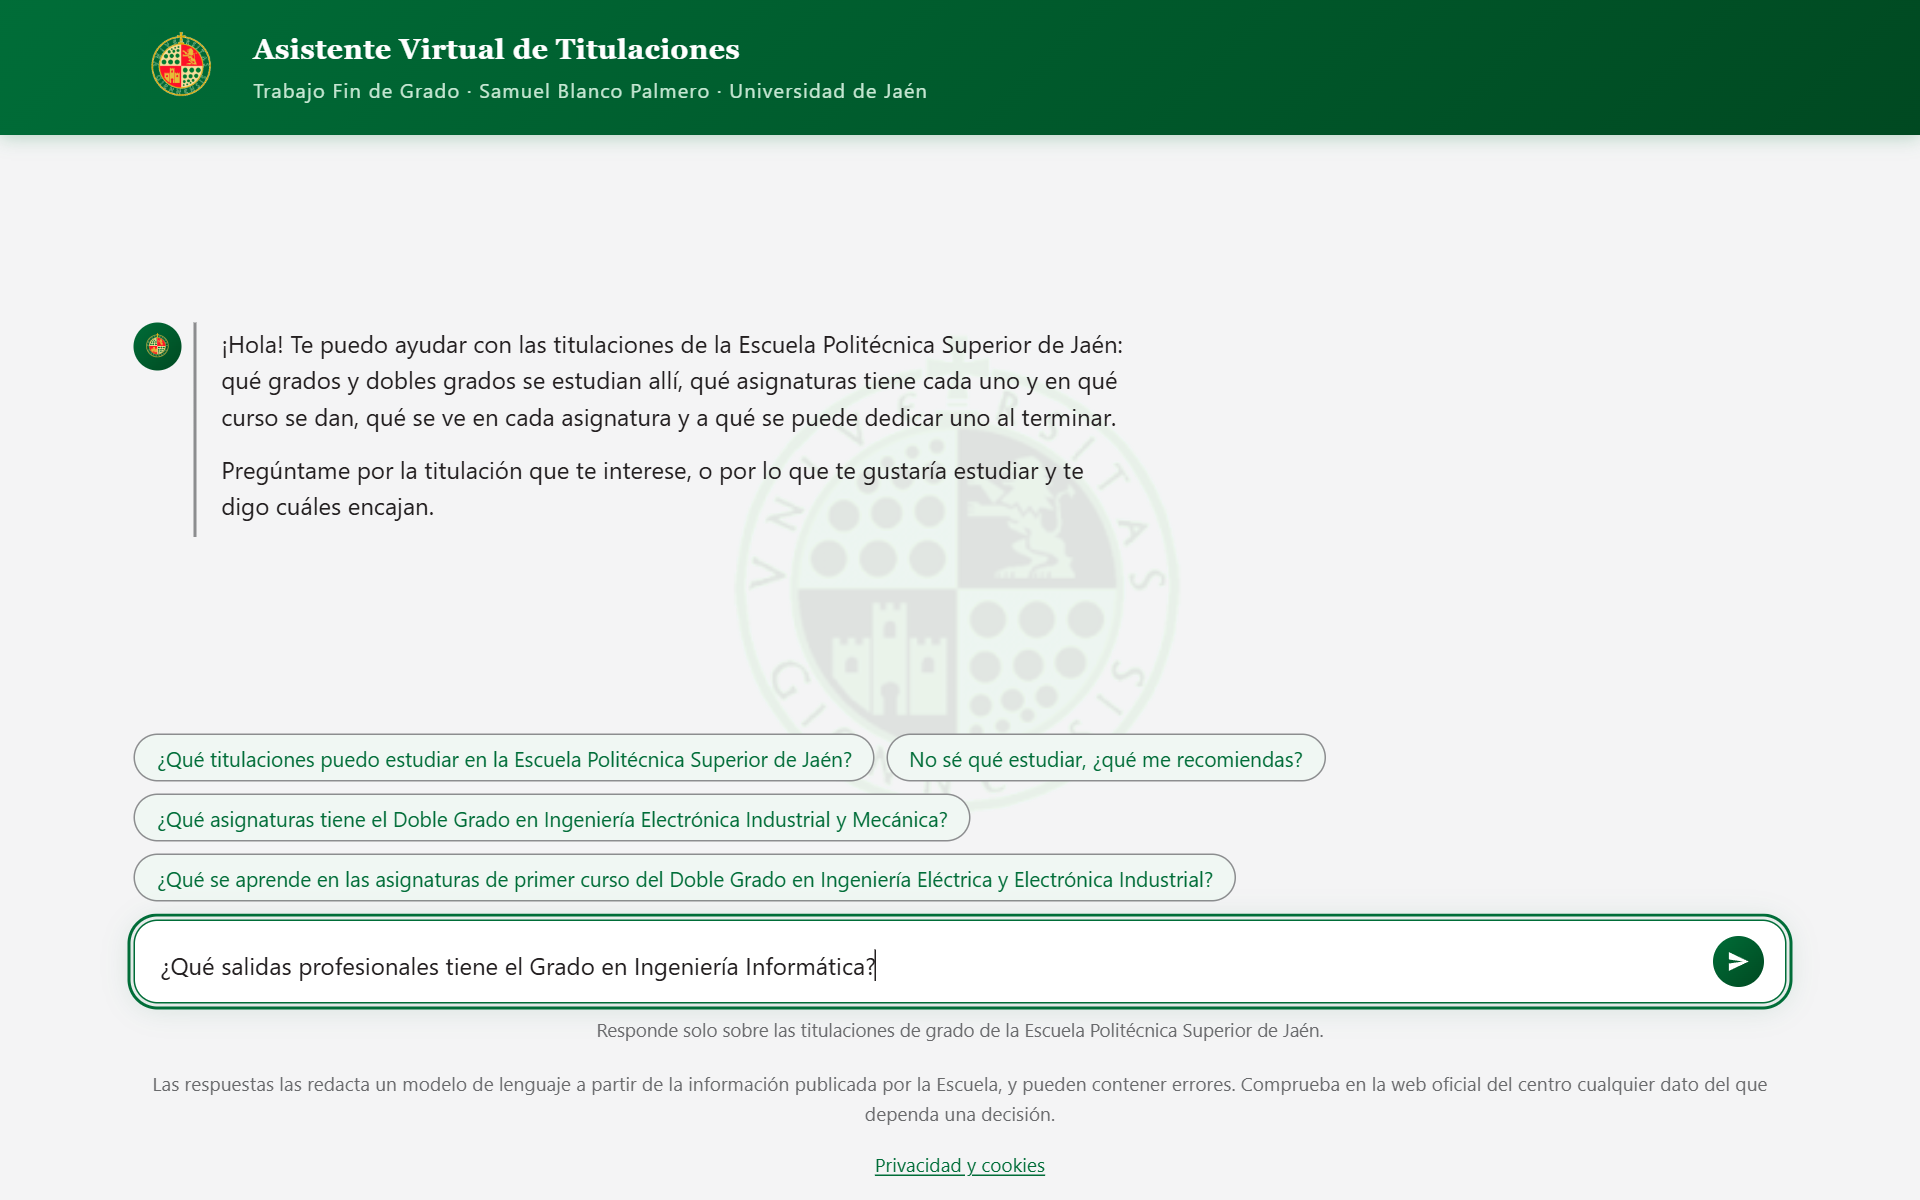
\includegraphics[width=\textwidth]{capturas/02_pregunta_escrita.png}
  \caption[Pregunta escrita en el cuadro de texto, lista para enviar.]{Pregunta escrita en el cuadro de texto, lista para enviar.}
  \label{fig:escrita}
\end{figure}

\subsection[Mientras esperas la respuesta]{Mientras esperas la respuesta}

La respuesta se prepara en dos pasos. Primero, el asistente busca en la información de la Escuela que tiene almacenada localmente. Mientras tanto verás el aviso «Buscando en la información de la Escuela» con un contador de segundos (Figura~\ref{fig:buscando}). Después, el modelo de lenguaje escribe la respuesta, que va apareciendo poco a poco junto a la palabra «escribiendo\ldots» (Figura~\ref{fig:redactando}).

Normalmente la respuesta llega en menos de un minuto, aunque las preguntas más complicadas o las respuestas largas pueden tardar más tiempo, todo dependiendo de los componentes y recursos que tenga tu equipo. La primera pregunta después de arrancar va algo más lenta, porque el modelo tiene que cargarse en memoria. Si la espera se alarga, la propia pantalla te avisa de que el modelo se ejecuta en tu equipo.

Mientras se prepara una respuesta no puedes enviar otra pregunta, y el botón de enviar se convierte en un botón de parar. Si lo pulsas, la consulta se detiene, aparece el mensaje «Consulta cancelada.» y tu pregunta vuelve al cuadro de texto por si quieres cambiarla.

\begin{figure}[H]
  \centering
  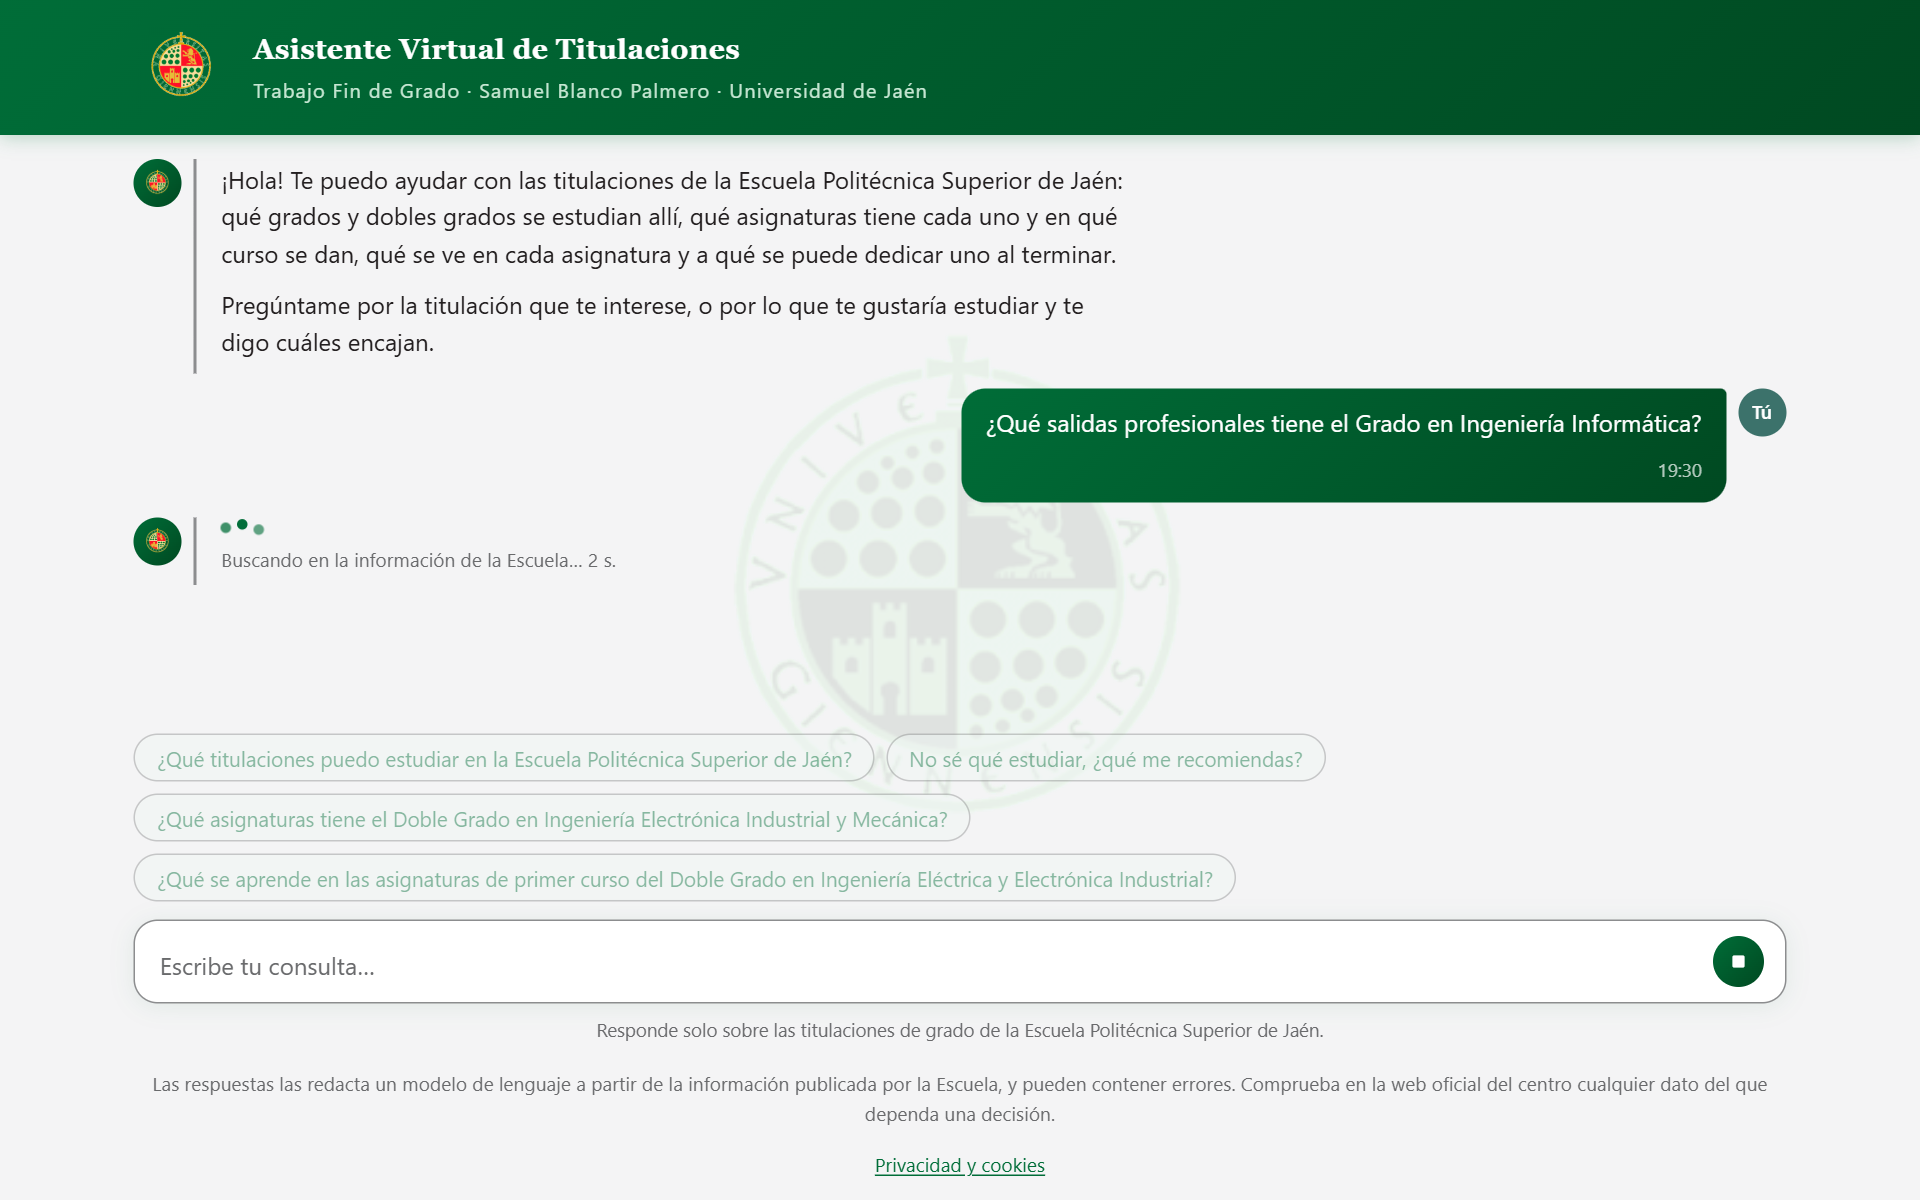
\includegraphics[width=\textwidth]{capturas/03_buscando.png}
  \caption[El asistente busca en la información de la Escuela.]{El asistente busca en la información de la Escuela. El botón de enviar se ha convertido en el de parar.}
  \label{fig:buscando}
\end{figure}

\begin{figure}[H]
  \centering
  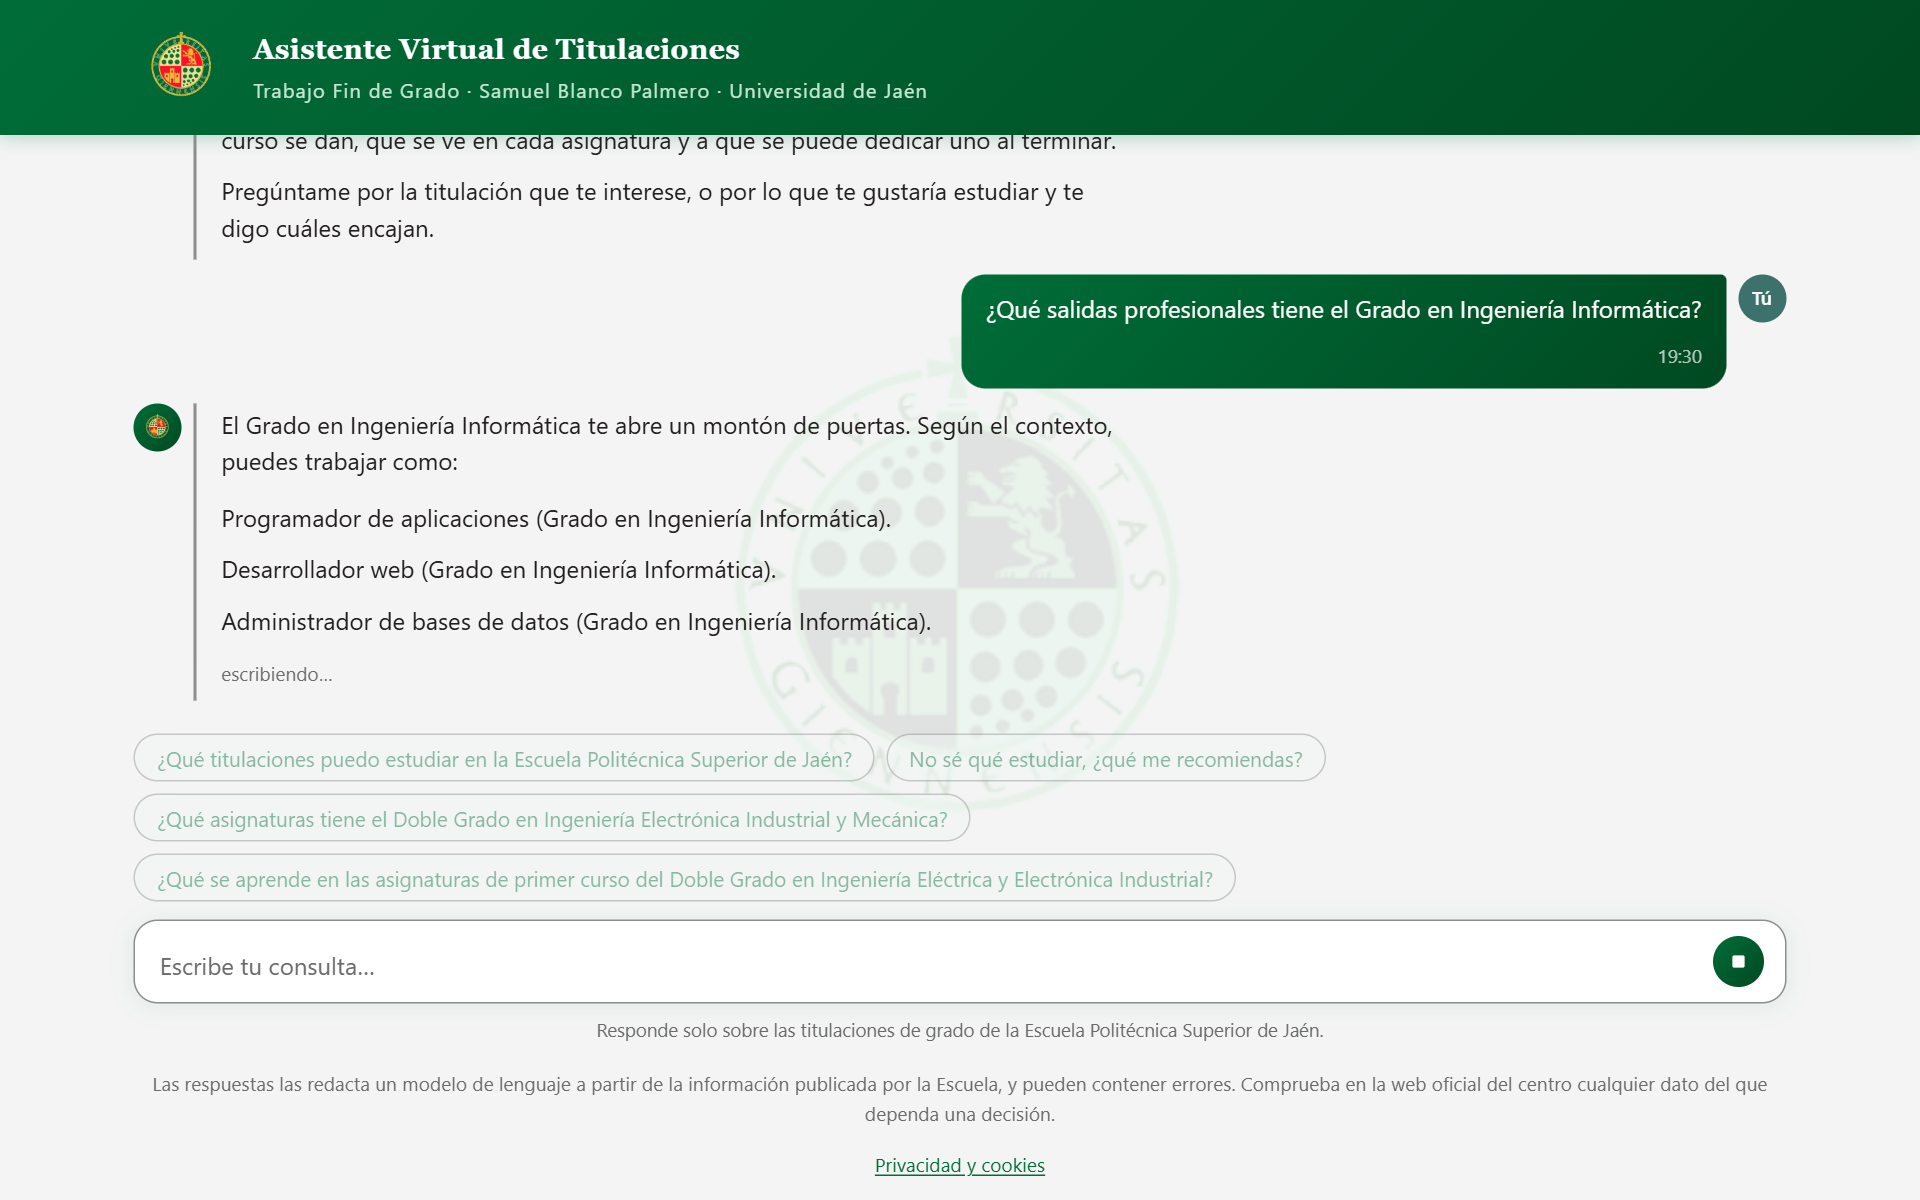
\includegraphics[width=\textwidth]{capturas/04_redactando.png}
  \caption[La respuesta va apareciendo poco a poco.]{La respuesta va apareciendo poco a poco mientras se escribe.}
  \label{fig:redactando}
\end{figure}

\subsection[La respuesta y sus fuentes]{La respuesta y sus fuentes}

Cuando la respuesta termina, debajo aparecen la hora, lo que ha tardado y un botón «Fuentes» con el número de documentos consultados entre paréntesis (Figura~\ref{fig:respuesta}).

\begin{figure}[H]
  \centering
  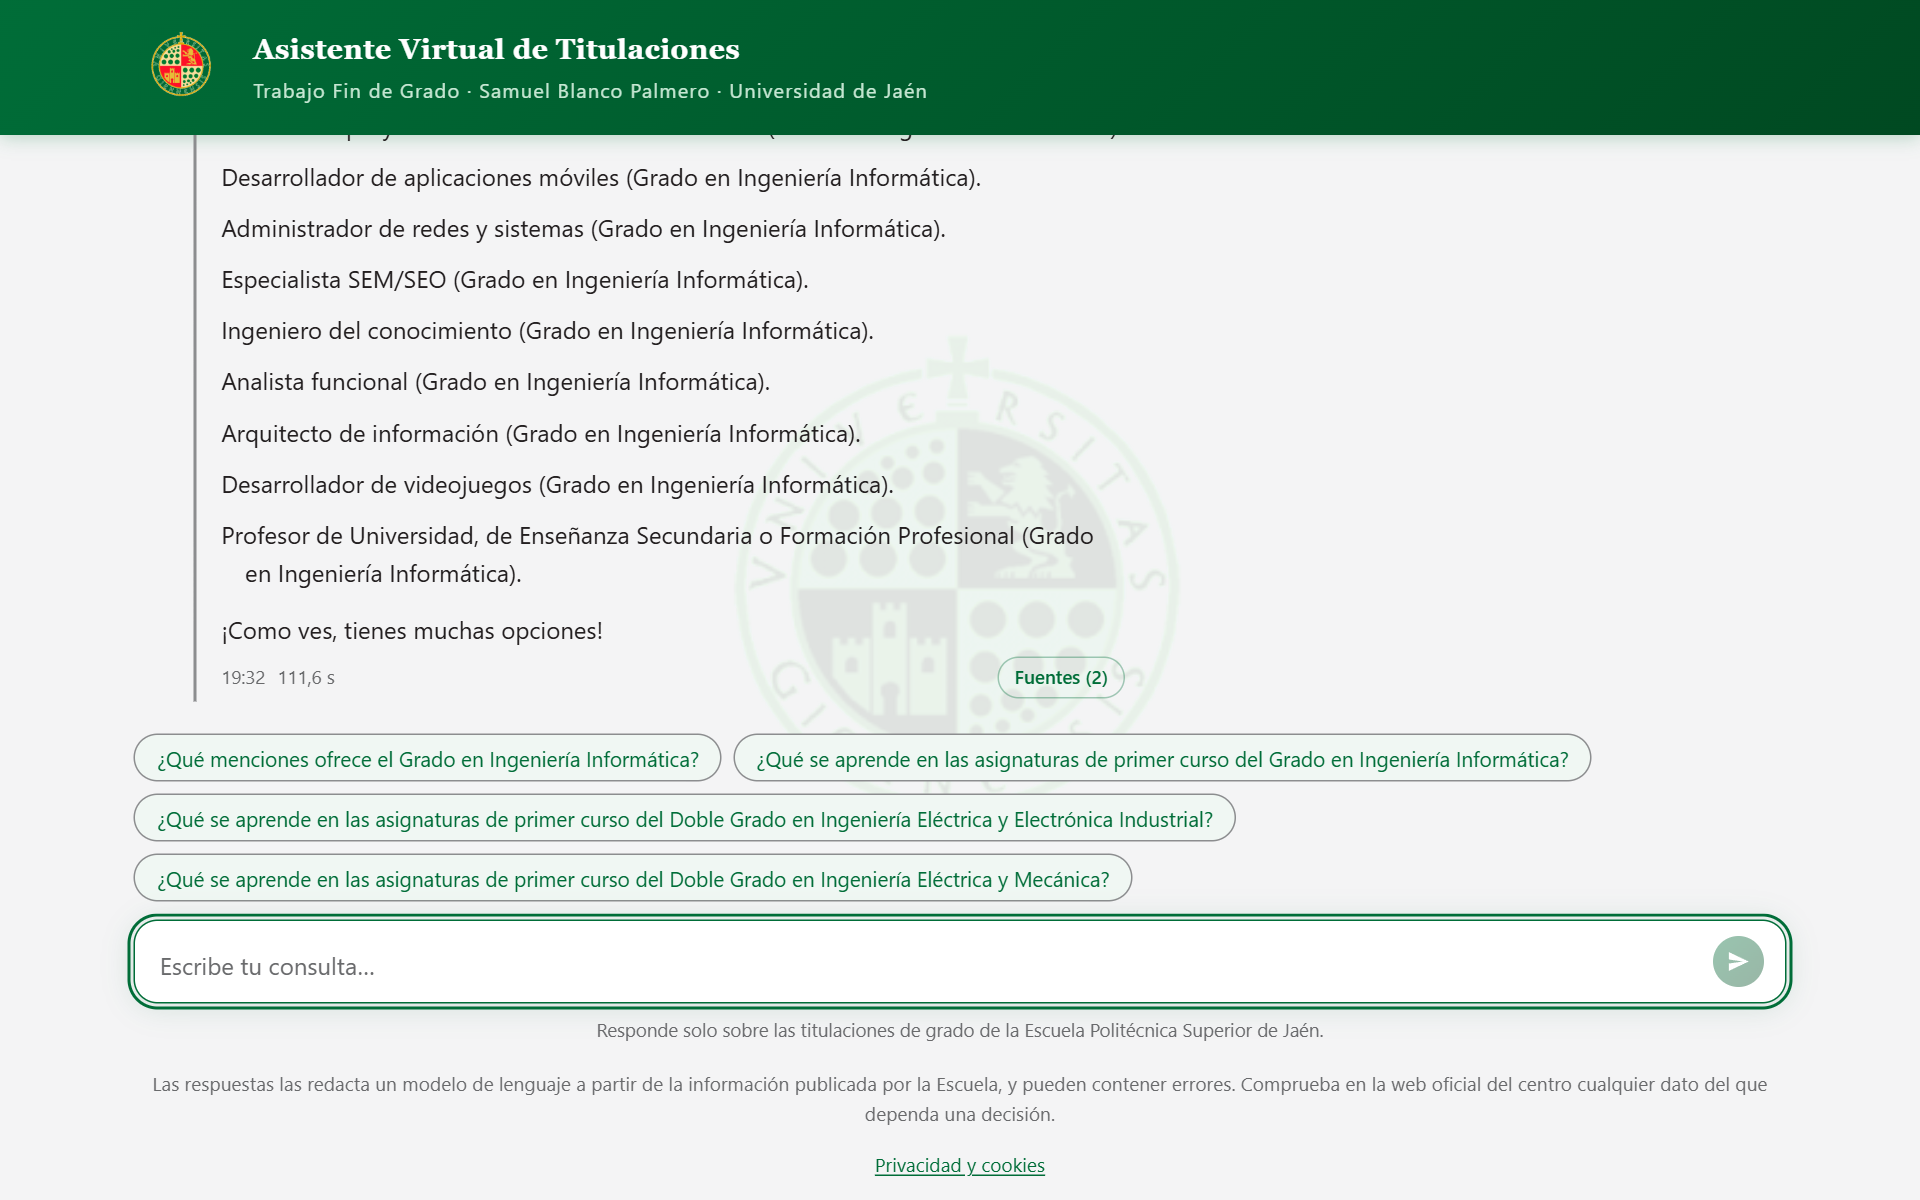
\includegraphics[width=\textwidth]{capturas/05_respuesta.png}
  \caption[Respuesta terminada, con la hora, lo que ha tardado y el botón de las fuentes.]{Respuesta terminada, con la hora, lo que ha tardado y el botón de las fuentes.}
  \label{fig:respuesta}
\end{figure}

Si pulsas el botón de fuentes se abre la ventana «Fuentes consultadas» (Figura~\ref{fig:fuentes}). Ahí aparecen los documentos de los que salen los fragmentos que se le pasaron al modelo para responder, agrupados por titulación y con su tipo (guía docente, plan de estudios, salidas profesionales, etc.). Si el documento tiene página en la web de la EPSJ, su título es un enlace para que puedas comprobar el dato original.

Ten en cuenta que, si un documento aparece en la lista, es porque se le dio al modelo, pero eso no quiere decir que el modelo haya usado todo lo que contiene. La ventana se cierra con el botón de cerrar o con la tecla Esc.

\begin{figure}[H]
  \centering
  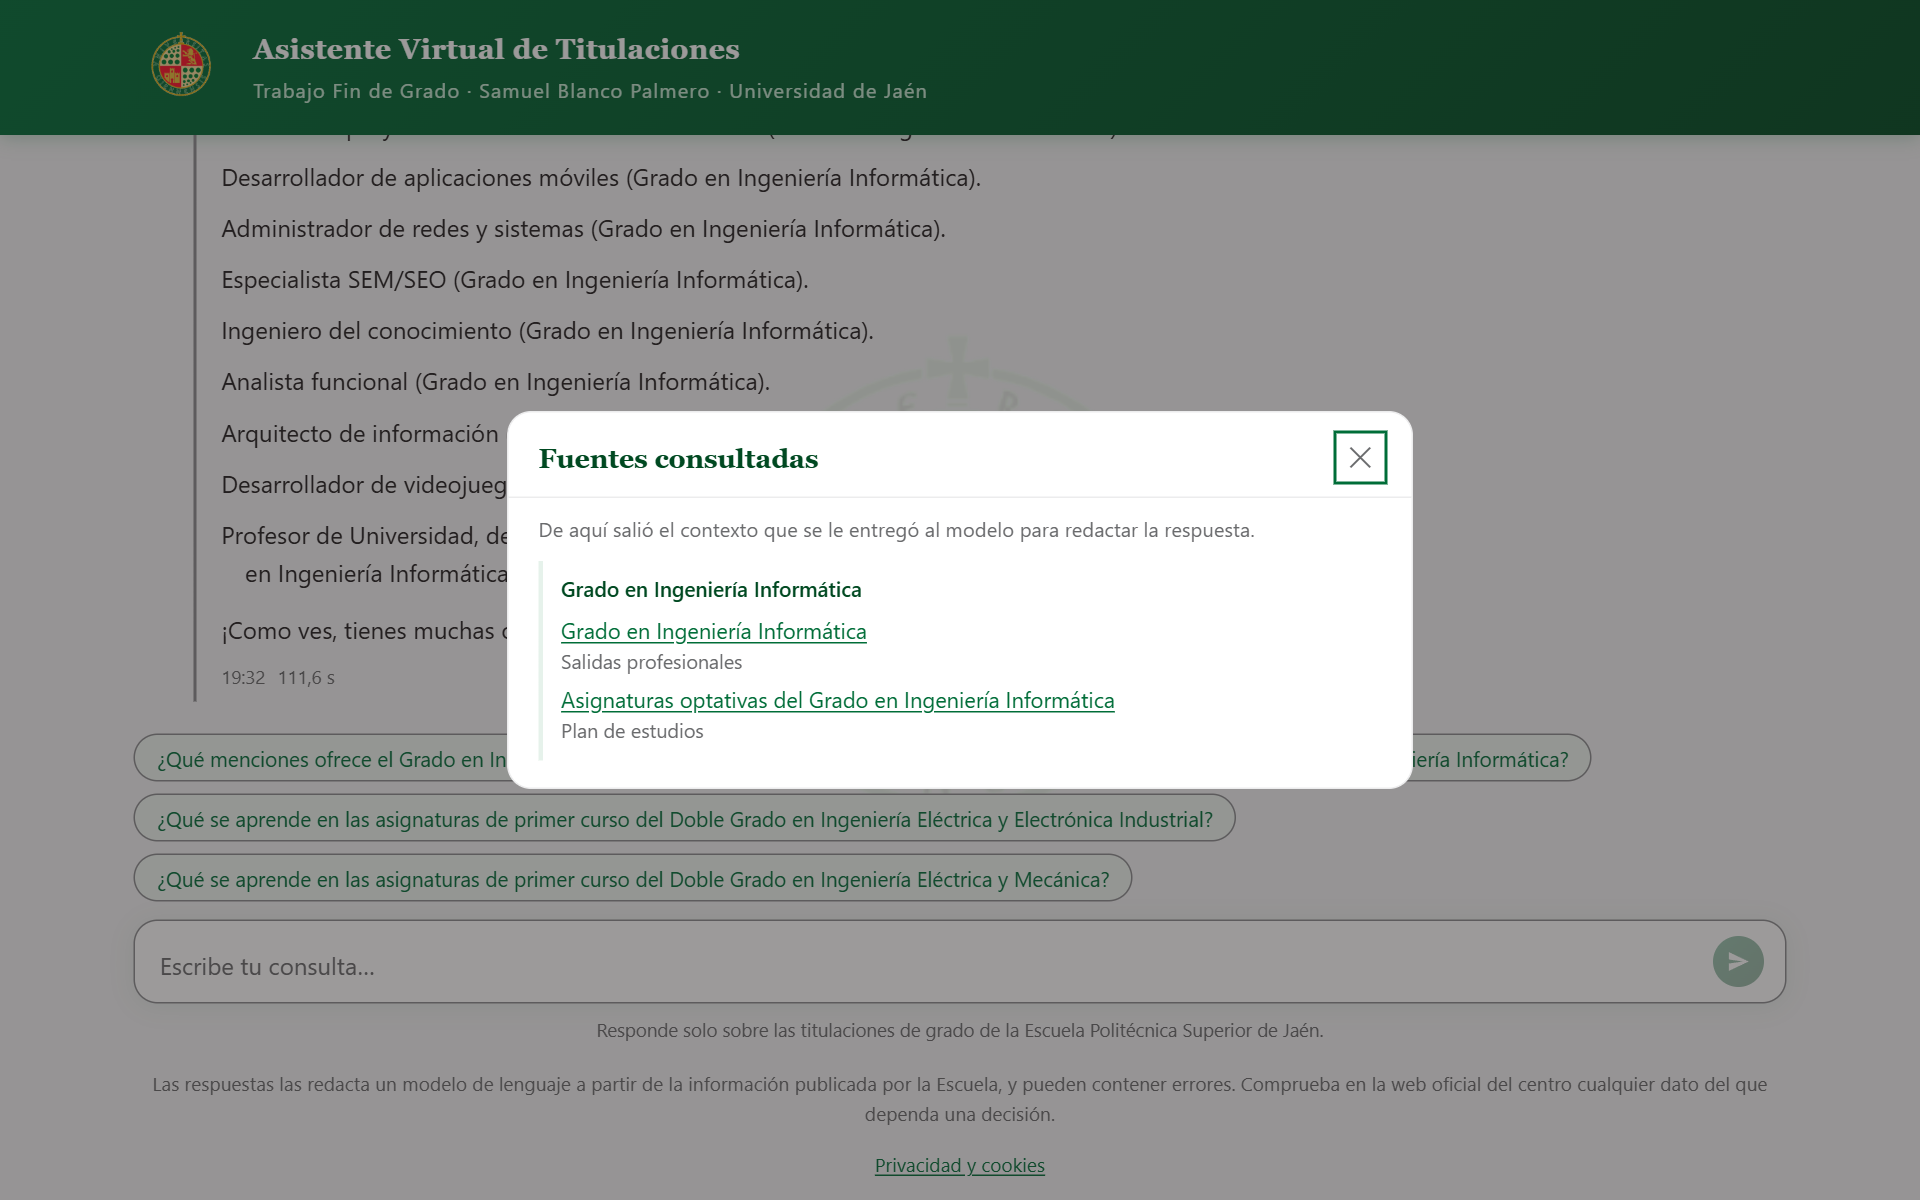
\includegraphics[width=\textwidth]{capturas/06_fuentes.png}
  \caption[Ventana con las fuentes consultadas.]{Ventana con las fuentes consultadas.}
  \label{fig:fuentes}
\end{figure}

% ---------------------------------------------------------------
\section[Seguir la conversación]{Seguir la conversación}

No hace falta que repitas el nombre de la titulación en cada pregunta. El asistente recuerda tus tres últimas preguntas a modo de contexto, su última respuesta y la titulación de la que estáis hablando. Por eso entiende preguntas de seguimiento como «¿Cuántos créditos tiene el trabajo fin de grado?» cuando antes estabas preguntando por el Grado en Ingeniería Informática (Figura~\ref{fig:seguimiento}).

Si quieres empezar de cero, recarga la página, ya que la conversación se borrará y el asistente olvidará todo lo anterior.

\begin{figure}[H]
  \centering
  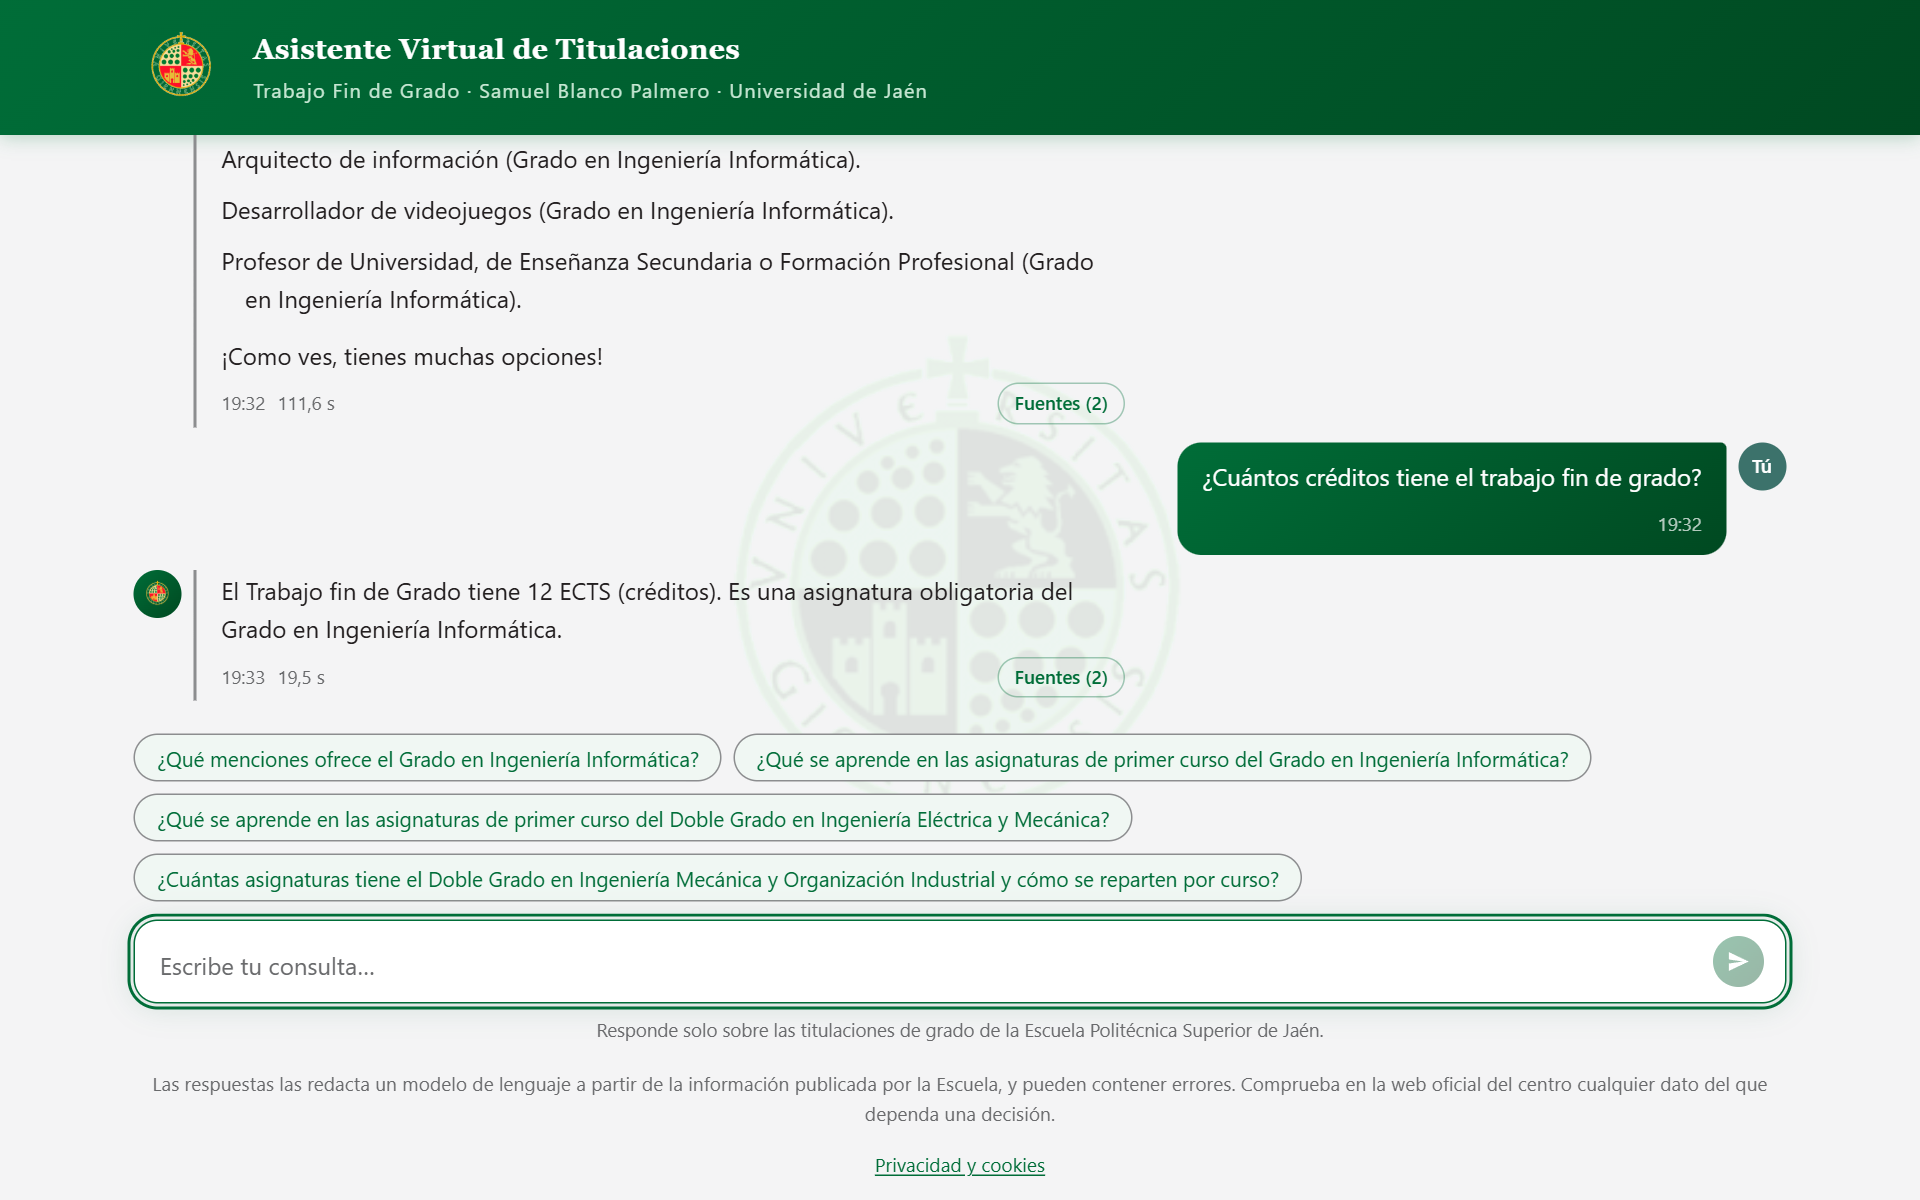
\includegraphics[width=\textwidth]{capturas/07_seguimiento.png}
  \caption[Una pregunta de seguimiento.]{Una pregunta de seguimiento: el asistente recuerda de qué titulación se estaba hablando.}
  \label{fig:seguimiento}
\end{figure}

% ---------------------------------------------------------------
\section[Pedir consejo]{Pedir consejo}

Además de responder preguntas concretas sobre las asignaturas, el asistente también te puede orientar si todavía no sabes qué estudiar. Si pulsas la sugerencia «No sé qué estudiar, ¿qué me recomiendas?», te resume en pocas líneas las titulaciones de la Escuela y te pregunta qué te gusta para afinar la recomendación (Figura~\ref{fig:consejo}). También puedes contarle directamente lo que te interesa, por ejemplo: «Me interesan la programación y las matemáticas, ¿qué titulación me recomiendas?».

Estos consejos salen de la información que publica la EPSJ, pero no son un test vocacional ni una evaluación hecha a tu medida. Antes de decidirte, mira con calma las asignaturas y el plan de estudios de las titulaciones que te sugiera.

\begin{figure}[H]
  \centering
  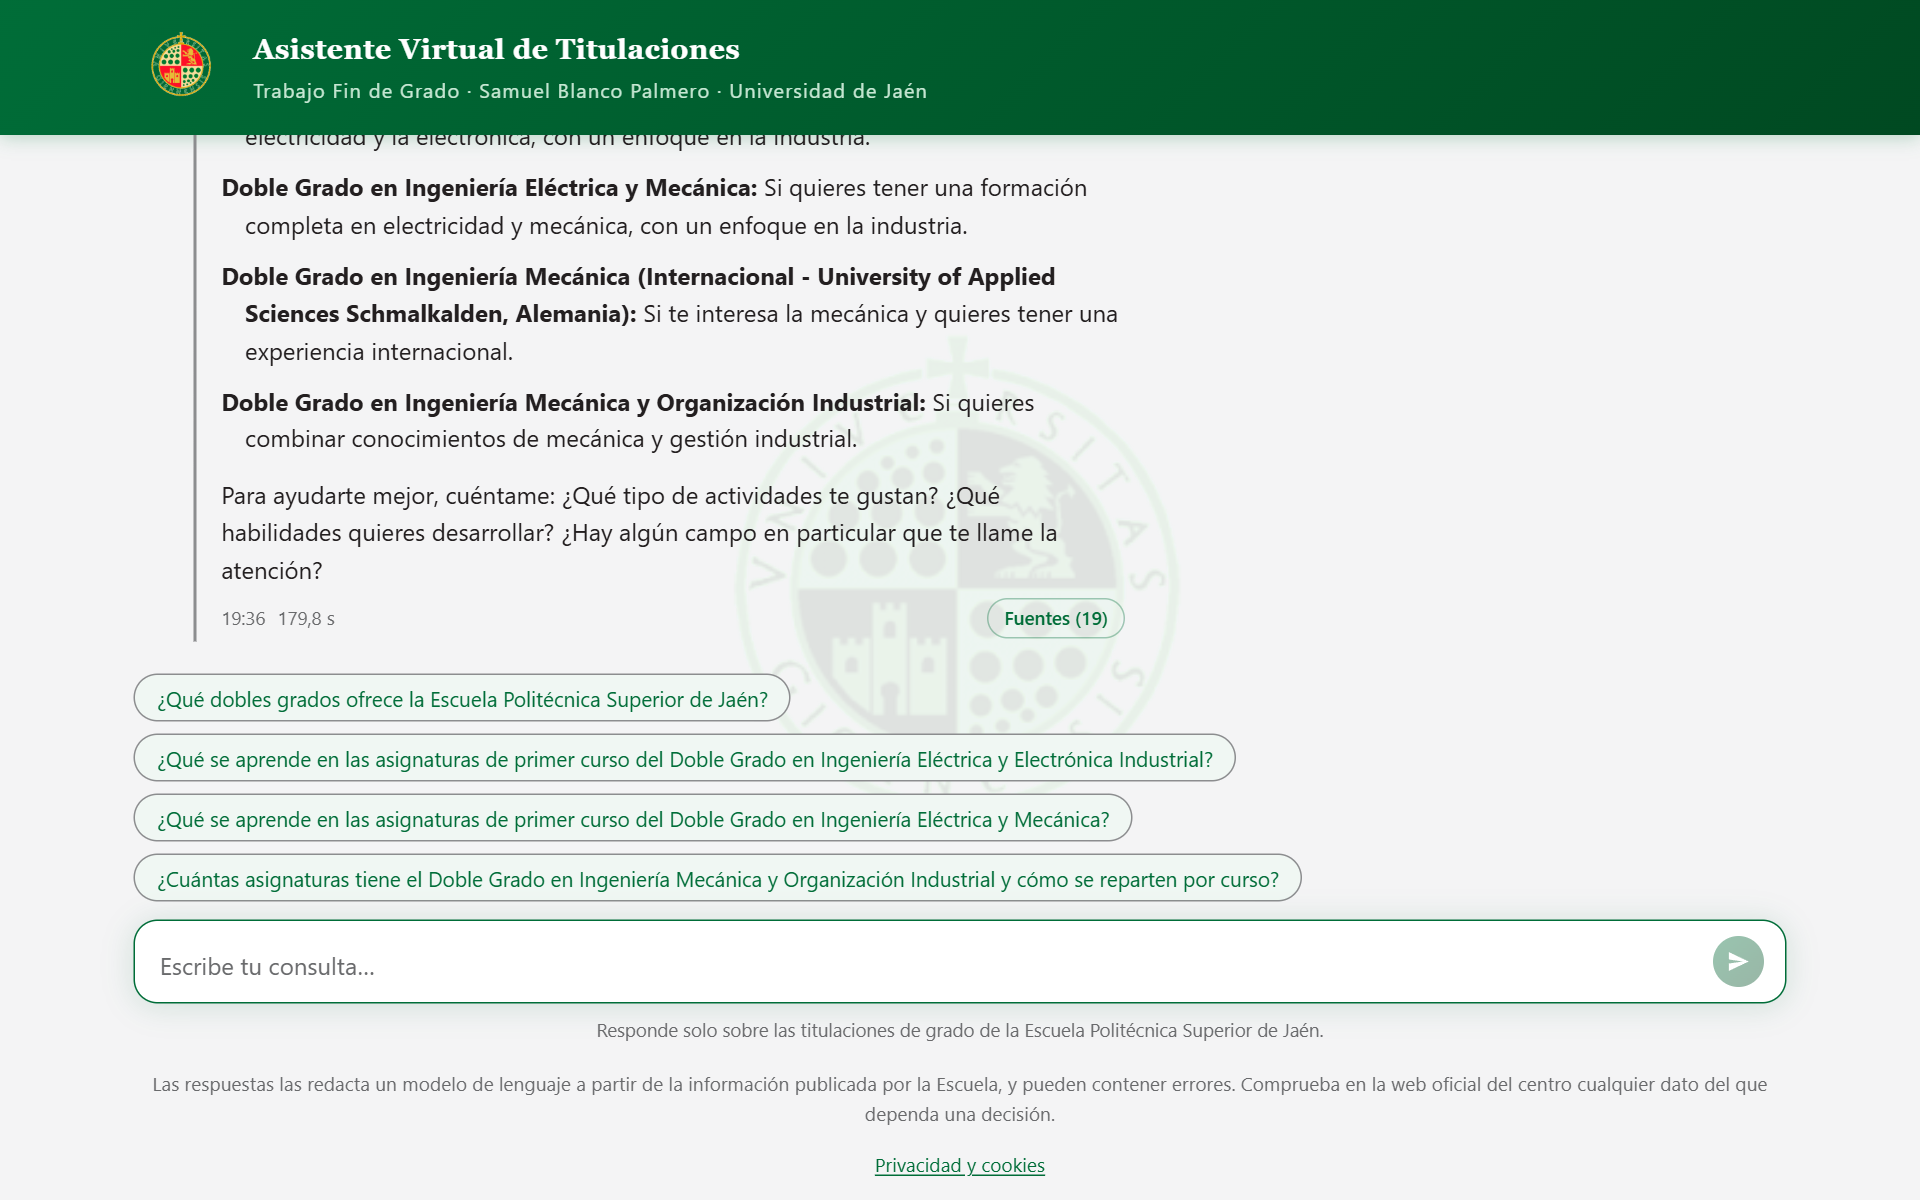
\includegraphics[width=\textwidth]{capturas/12_consejo_sugerencia.png}
  \caption[Respuesta a la sugerencia «No sé qué estudiar, ¿qué me recomiendas?».]{Respuesta a la sugerencia «No sé qué estudiar, ¿qué me recomiendas?».}
  \label{fig:consejo}
\end{figure}

% ---------------------------------------------------------------
\section[Lo que el asistente no responde]{Lo que el asistente no responde}

El asistente solo habla de los grados de la Escuela Politécnica Superior de Jaén. Si preguntas por otra universidad o por otro centro, aunque sea de la propia Universidad de Jaén, te contesta al momento que de eso no puede informarte y te remite a la web de ese centro, en lugar de inventarse nada (Figura~\ref{fig:ajena}). Como es una respuesta fija, no lleva fuentes. Las preguntas que no tienen nada que ver con los estudios también se rechazan, aunque no siempre con esta misma respuesta.

El asistente también está hecho para no dar datos que la Escuela no haya publicado. Si la guía docente de una asignatura no está en la web, te lo dirá en lugar de imaginarse lo que pone. Y no tiene información sobre el profesorado (nombres, correos o despachos): se dejó fuera a propósito para proteger su privacidad y cumplir la ley de protección de datos.

\begin{figure}[H]
  \centering
  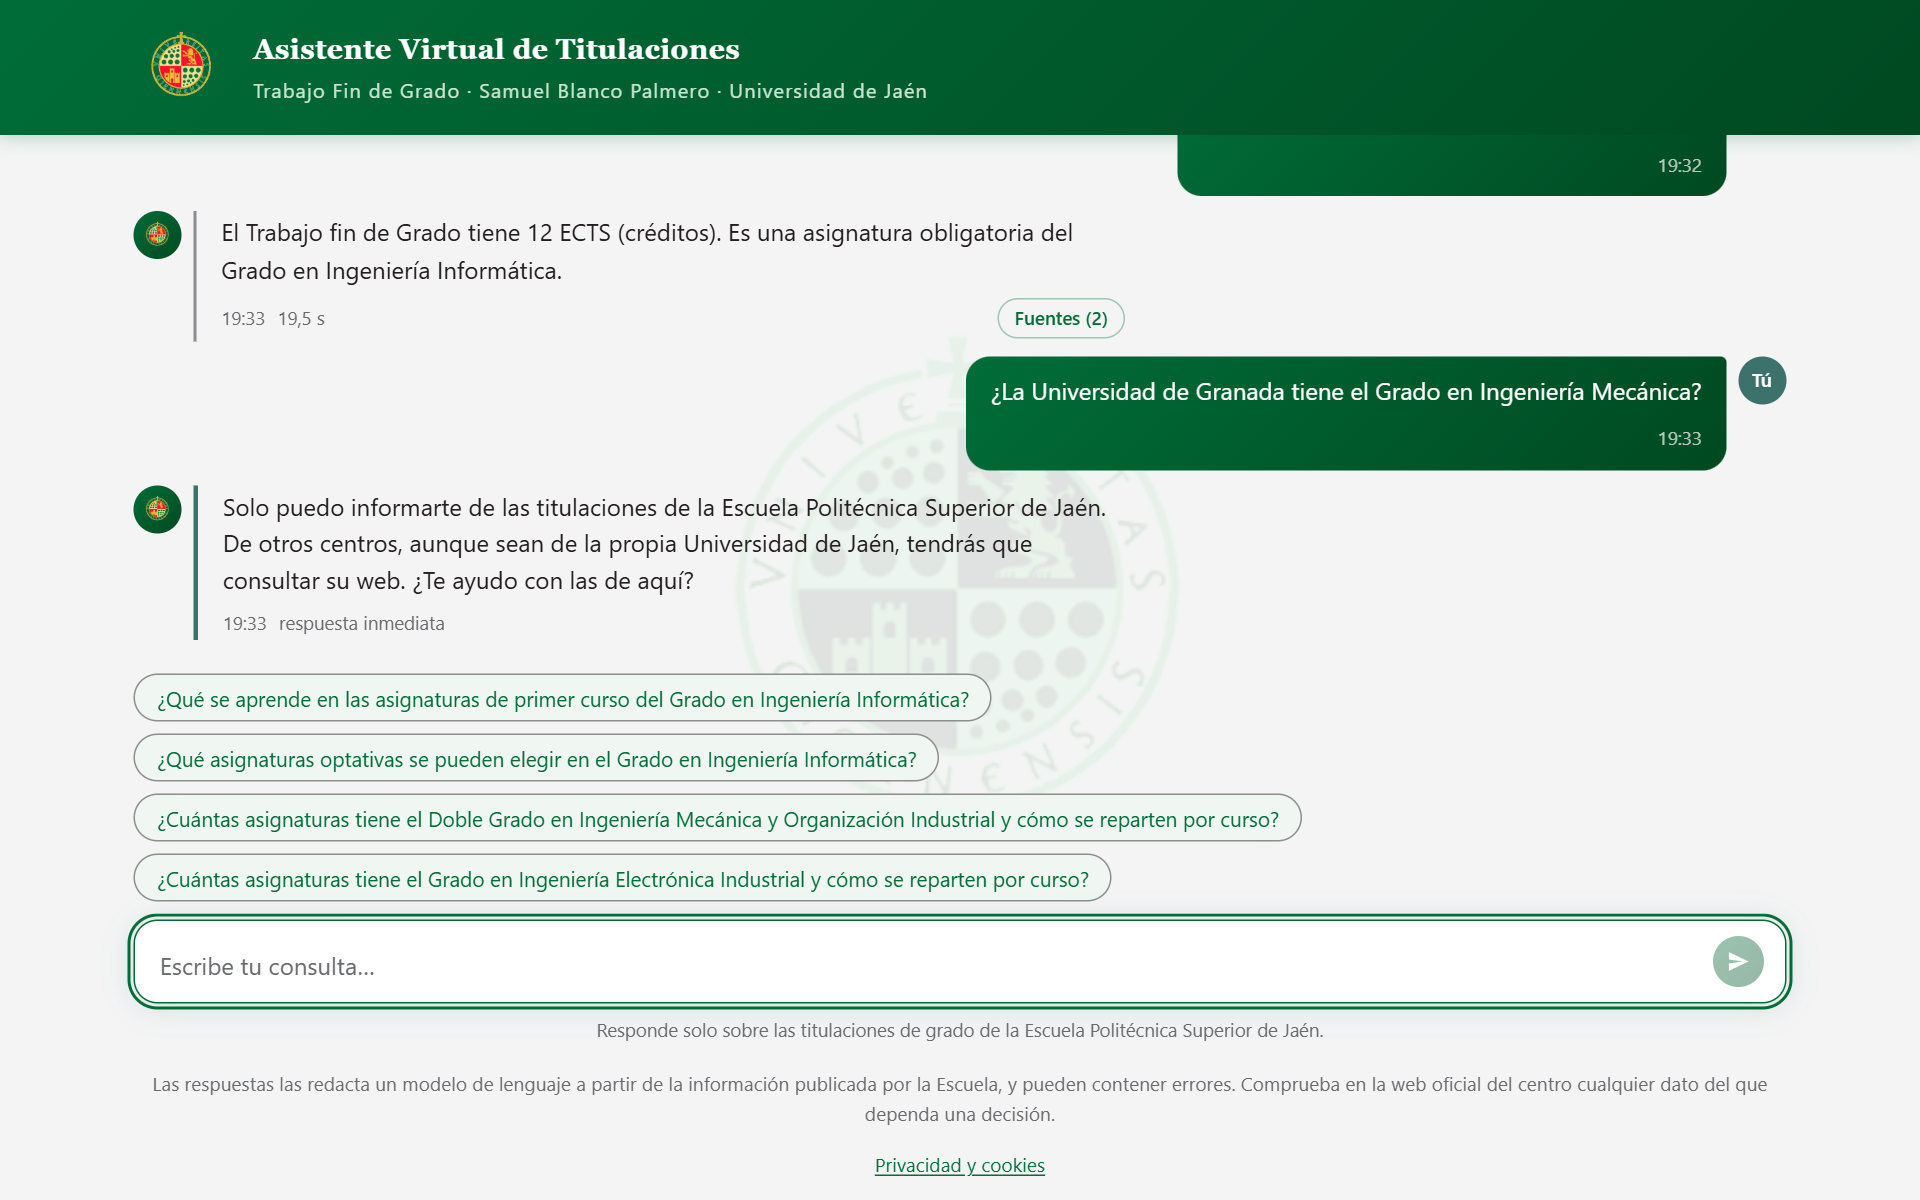
\includegraphics[width=\textwidth]{capturas/08_fuera_de_ambito.png}
  \caption[Respuesta a una pregunta sobre otra universidad.]{Respuesta a una pregunta sobre otra universidad.}
  \label{fig:ajena}
\end{figure}



% ---------------------------------------------------------------
\section[Privacidad]{Privacidad}

El asistente está pensado para proteger tus datos:

\begin{itemize}
  \item \textbf{Sin cuentas ni datos personales:} No tienes que registrarte ni dar ningún dato tuyo. Aun así, no escribas datos personales en las preguntas, como tu nombre, tu DNI, tu dirección o tu teléfono.
  \item \textbf{Sin rastreadores:} La aplicación no usa cookies, no guarda nada en tu navegador y no se conecta a servidores de publicidad ni carga nada de fuera.
  \item \textbf{Todo en tu ordenador:} Las búsquedas y las respuestas se hacen en tu propio equipo, y tus preguntas no se envían a ninguna empresa ni a ningún servicio en la nube.
  \item \textbf{La conversación no se guarda:} La aplicación solo recuerda la conversación mientras la usas, y esta se borra del todo al recargar la página o al parar el asistente.
  \item \textbf{Registro solo para pruebas:} El asistente tiene una opción (\texttt{--registrar}) que guarda las conversaciones para analizarlas en el trabajo a modo de monitorización para mejorar la aplicación. Por defecto está desactivada.
\end{itemize}

Todo esto, y también cómo ejercer tus derechos sobre tus datos, está explicado con más detalle en la página «Privacidad y cookies», enlazada al pie de la pantalla (Figura~\ref{fig:privacidad}).

\begin{figure}[H]
  \centering
  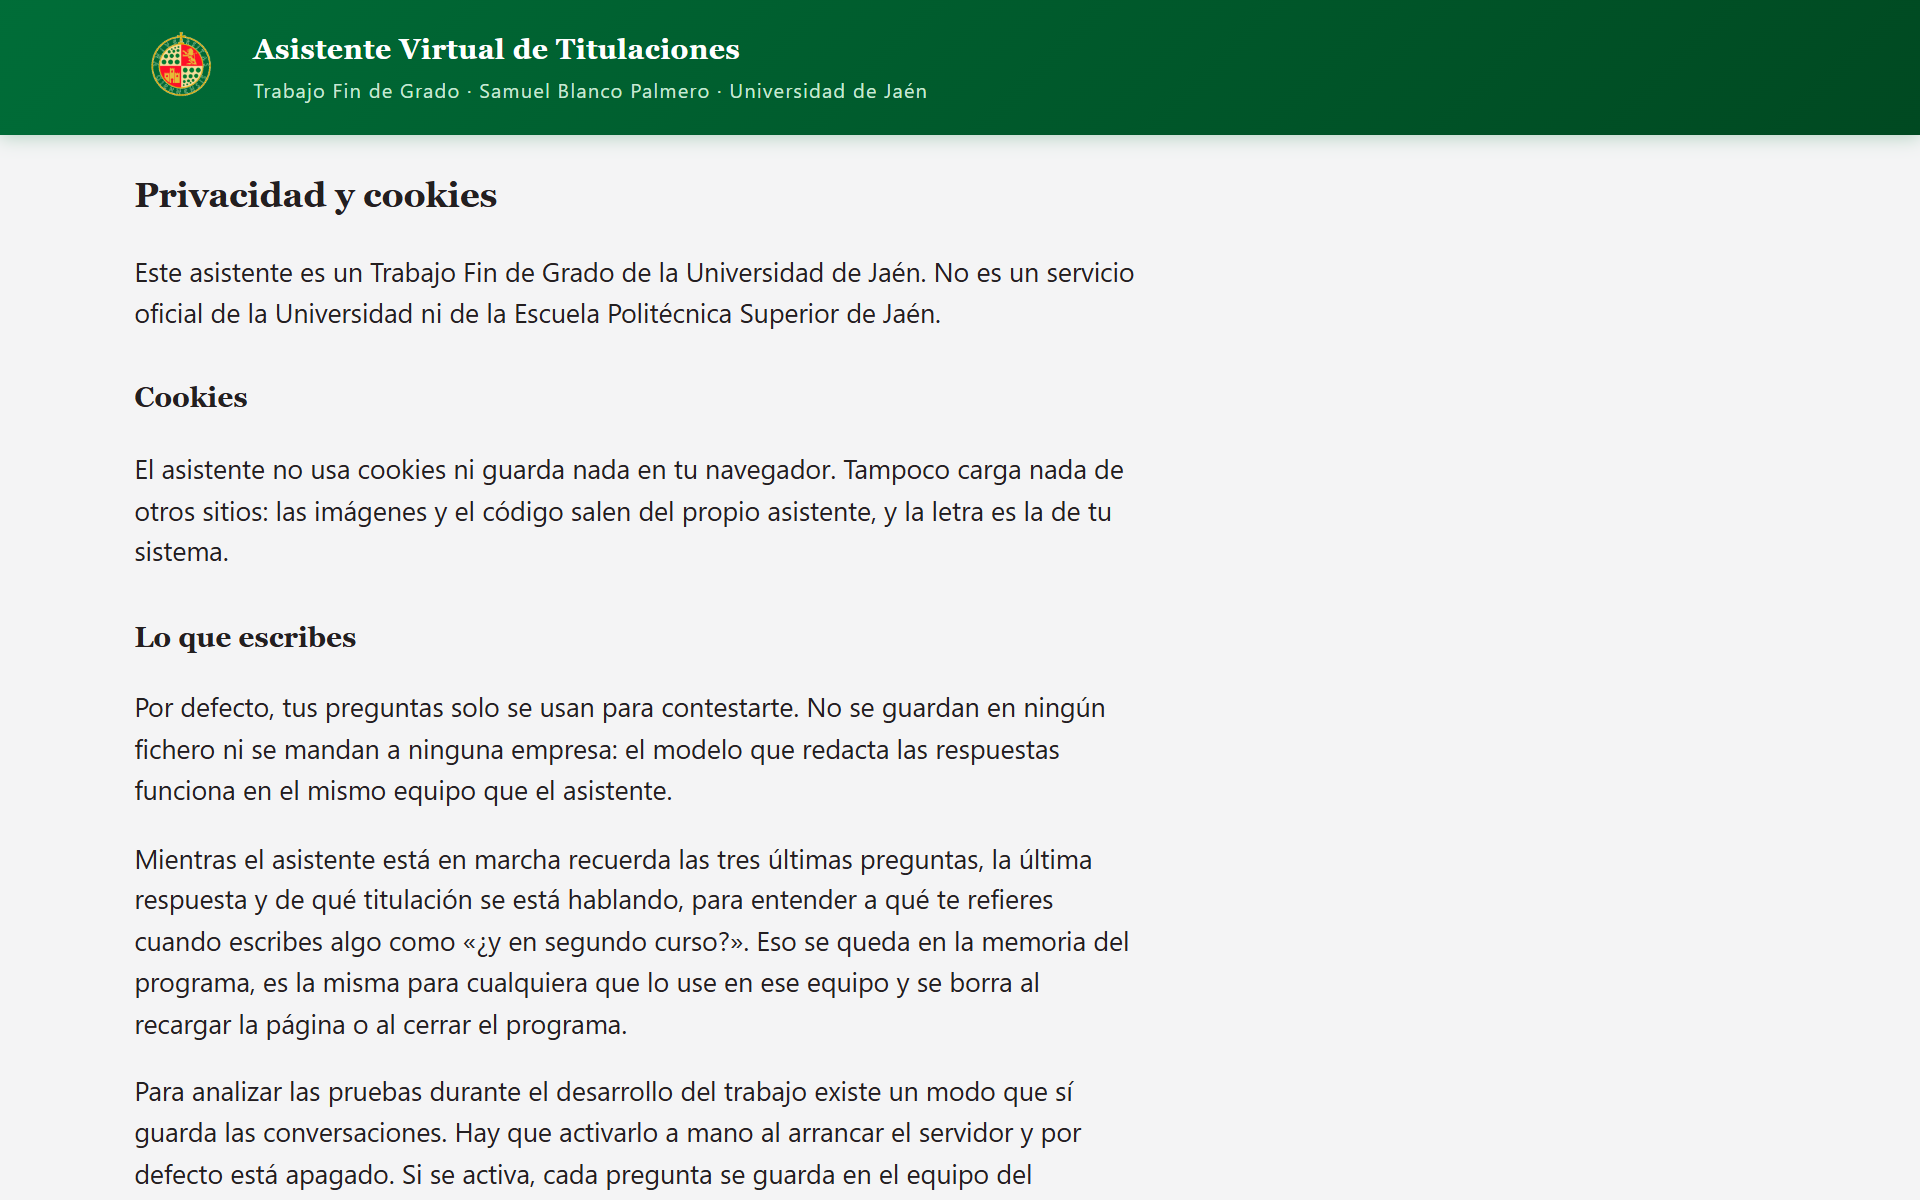
\includegraphics[width=\textwidth]{capturas/10_privacidad.png}
  \caption[La página de privacidad y cookies.]{La página de privacidad y cookies.}
  \label{fig:privacidad}
\end{figure}

% ---------------------------------------------------------------
\section[Errores comunes]{Errores comunes}

Estos son los problemas más habituales al ponerlo en marcha o al usarlo, y cómo resolverlos:

\begin{description}[style=nextline]
  \item[La página no carga en el navegador.]
    El asistente no está arrancado o se ha parado. Arráncalo como se explica en la Sección~\ref{sec:arrancar} y comprueba que la dirección sea exactamente \texttt{http://127.0.0.1:8000}.

  \item[El asistente no arranca y dice que falta el índice.]
    No encuentra el índice en \texttt{data/indice\_lance}. Sigue los pasos de la Sección~\ref{sec:instalacion} para crearlo.

  \item[Aparece el aviso «No se ha podido obtener una respuesta».]
    Normalmente es que Ollama no responde o se ha cerrado. Comprueba que Ollama está en marcha y vuelve a enviar la pregunta.

  \item[Las respuestas tardan mucho tiempo.]
    El modelo \texttt{gemma3:12b} necesita mucha memoria, tanto RAM como de la tarjeta gráfica. Si a la vez tienes abiertos programas que gastan mucha memoria, como un navegador con muchas pestañas, irá bastante más lento. Cierra lo que no estés usando.

  \item[El asistente dice que no tiene esa información.]
    Pasa cuando lo que preguntas no está en la información oficial que publica la EPSJ, por ejemplo si la guía docente de ese curso todavía no se ha publicado. También puede ser que la pregunta sea demasiado general: prueba a escribirla otra vez diciendo la titulación y la asignatura.
\end{description}

\end{document}
